\chapter{METODOLOGI}
\label{chap:3}

% Ubah bagian-bagian berikut dengan isi dari desain dan implementasi

\section{Data dan Peralatan}
\label{sec:31}

\subsection{Dataset}
\label{sec:311}
Data yang digunakan dalam penelitian ini adalah data yang diperoleh dari Diabetic Retinopathy Analisis Grand challenge, berupa citra OCT-\emph{Angiography}.
Untuk persebaran data yang digunakan pada penelitian ini, terdapat pada tabel \ref{table:Datasettraining}

	\begin{figure}[hbtp]
		\centering
		\subfloat[\centering Non-DR]{{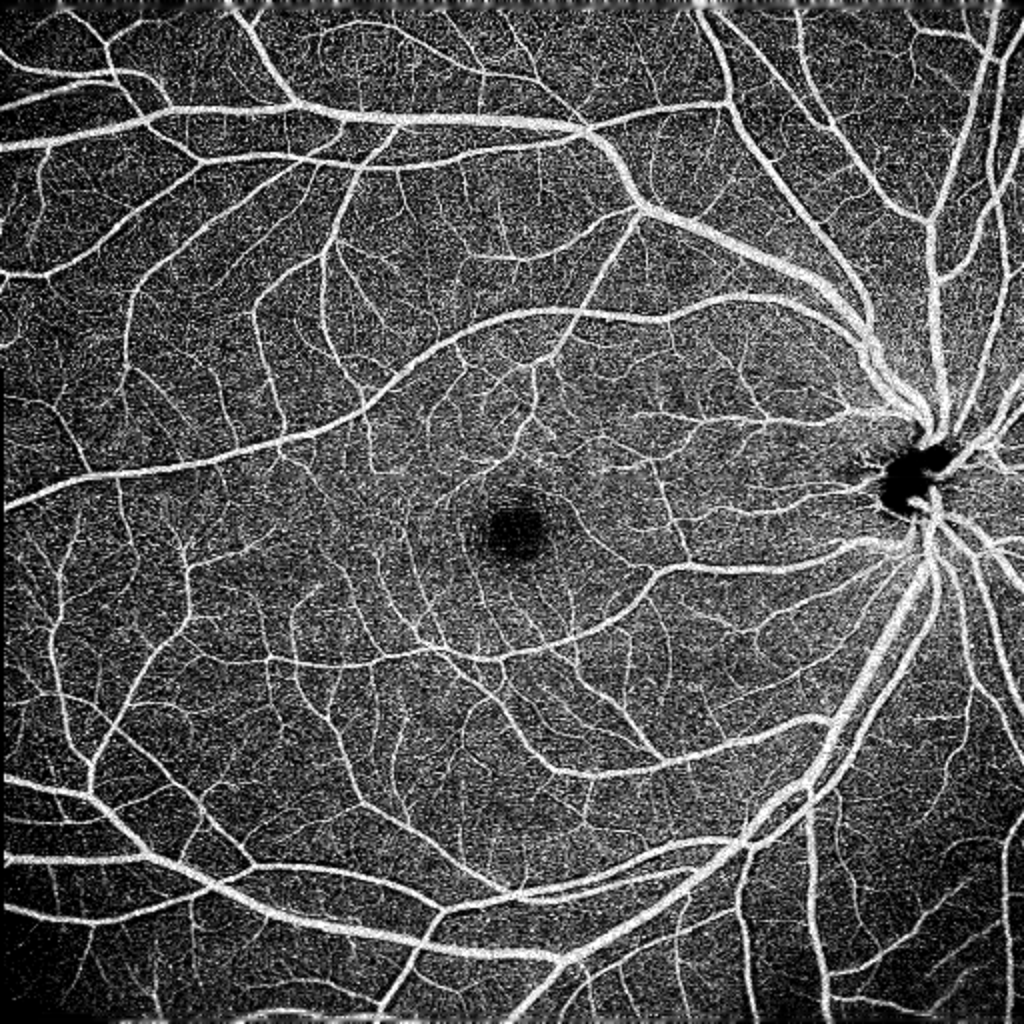
\includegraphics[width=5cm]{gambar/non-DR.png} }}%
		\subfloat[\centering NPDR]{{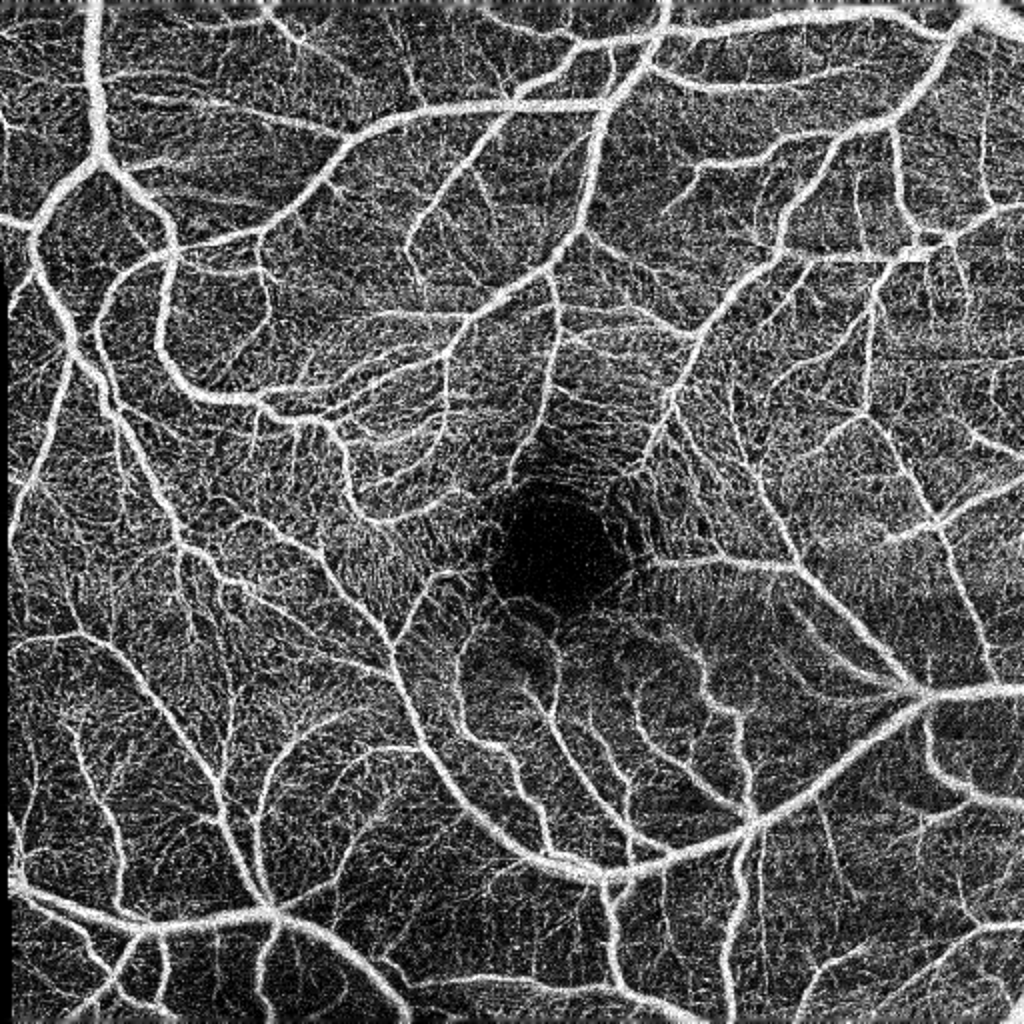
\includegraphics[width=5cm]{gambar/NPDR.png} }}%
		\subfloat[\centering PDR]{{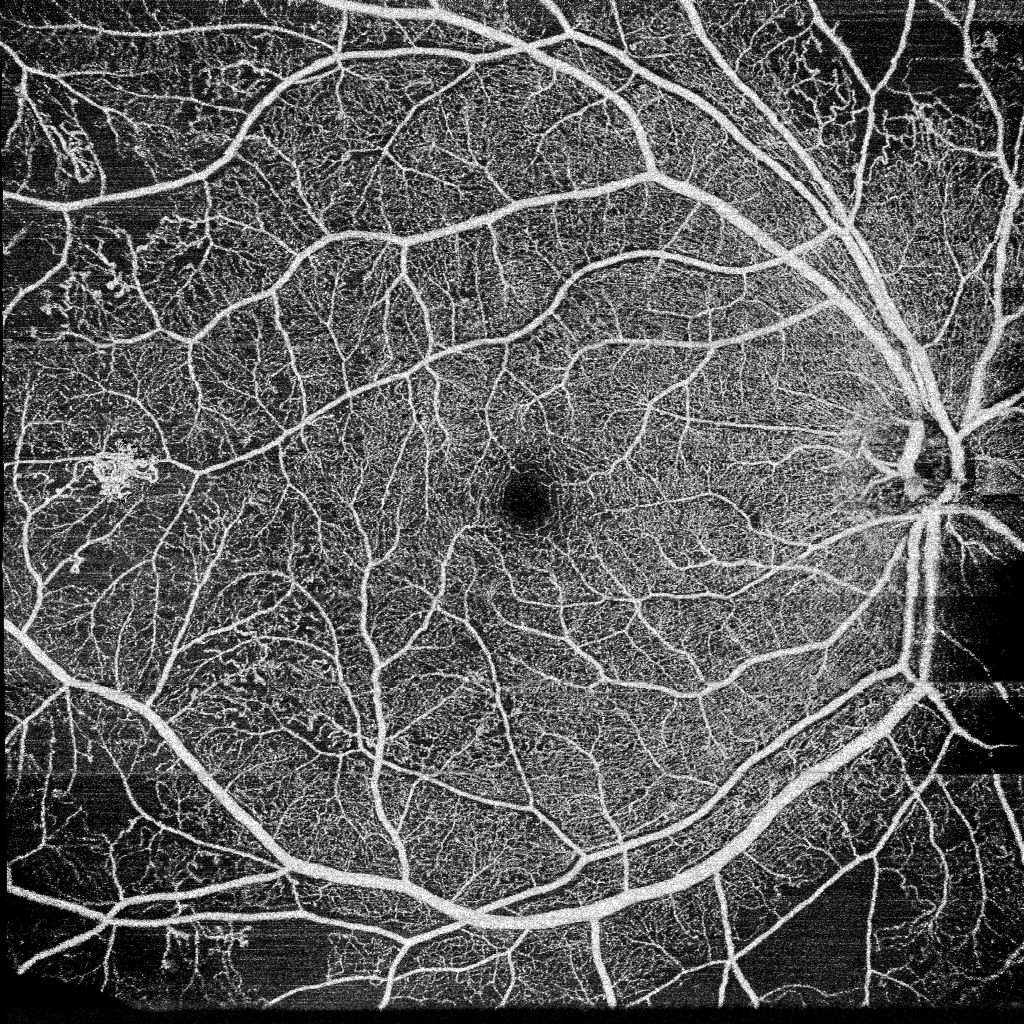
\includegraphics[width=5cm]{gambar/PDR.png} }}%
		\caption{Contoh Data Citra Retina}
		\label{fig:sampleDataset}
	\end{figure}
Gambar yang diberikan adalah foto fundus retina yang digunakan untuk evaluasi retinopati diabetik. Foto ini menunjukkan detail dari jaringan pembuluh darah retina, disk optik, dan area makula. Berikut adalah deskripsi rinci dari gambar tersebut:
	\begin{itemize}
		\item \textbf{Struktur Vaskular}: Jaringan pembuluh darah yang jelas terlihat memancar dari disk optik. Pembuluh darah tampak menonjol dan tersebar di seluruh retina.
		\item \textbf{Makula}: Terdapat titik gelap yang terlihat di dekat makula, yang mungkin menunjukkan perubahan retina.
	\end{itemize}
Retinopati diabetik dapat dikategorikan berdasarkan tingkat keparahannya sebagai berikut:

	\begin{enumerate}
		\item Non-DR (0): Non-Diabetic Retinopathy

		\textbf{Karakteristik}: Tidak ada tanda-tanda retinopati diabetik. Retina tampak normal tanpa mikroaneurisma, pendarahan, atau eksudat keras.
		\item NPDR (1): Non-Proliferative Diabetic Retinopathy.

		\textbf{Karakteristik}:
		\begin{itemize}
			\item Kehadiran mikroaneurisma (lesi kecil bulat).\
			\item Pendarahan retina (bercak gelap kecil).
			\item Eksudat keras (bintik-bintik putih terang).
			\item Tidak ada neovaskularisasi.
		\end{itemize}
		\item PDR (2): Proliferative Diabetic Retinopathy

		\textbf{Karakteristik}:
		\begin{itemize}
			\item Kehadiran neovaskularisasi (pertumbuhan pembuluh darah baru yang abnormal).
			\item Mungkin ada pendarahan vitreous (ke dalam humor vitreous mata).
			\item Menunjukkan kondisi yang lebih parah dan berisiko tinggi terhadap kehilangan penglihatan.
		\end{itemize}
	\end{enumerate}

Informasi Dataset dari Tantangan DRAC
Dataset yang digunakan untuk pelatihan dan pengujian terdiri dari:

	\begin{itemize}
		\item Set Pelatihan: 611 gambar
		\item Set Uji: 386 gambar
	\end{itemize}
Gambar-gambar pada set pelatihan, kemudian dipisah kembali menjadi dua set, yaitu set untuk pelatihan dan set untuk validasi dengan jumlah sesuai pada tabel \ref{table:Datasettraining}

\begin{table}[hbtp]
	\begin{center}
	\caption{Tabel distribusi Set untuk Pelatihan dan Validasi}
	\label{table:Datasettraining}
	\begin{tabular}{|l|l|l|l|}
		\hline
		\rowcolor[HTML]{C0C0C0} 
		Label                                                & Klasifikasi & Jumlah & Total                                         \\ \hline
		\rowcolor[HTML]{FFFFFF} 
		\cellcolor[HTML]{FFFFFF}                             & non-DR      & 263    & \cellcolor[HTML]{FFFFFF}                      \\ \cline{2-3}
		\rowcolor[HTML]{FFFFFF} 
		\cellcolor[HTML]{FFFFFF}                             & NPDR        & 169    & \cellcolor[HTML]{FFFFFF}                      \\ \cline{2-3}
		\rowcolor[HTML]{FFFFFF} 
		\multirow{-3}{*}{\cellcolor[HTML]{FFFFFF}Training}   & PDR         & 56     & \multirow{-3}{*}{\cellcolor[HTML]{FFFFFF}488} \\ \hline
		\rowcolor[HTML]{FFFFFF} 
		\cellcolor[HTML]{FFFFFF}                             & non-DR      & 66     & \cellcolor[HTML]{FFFFFF}                      \\ \cline{2-3}
		\rowcolor[HTML]{FFFFFF} 
		\cellcolor[HTML]{FFFFFF}                             & NPDR        & 43     & \cellcolor[HTML]{FFFFFF}                      \\ \cline{2-3}
		\rowcolor[HTML]{FFFFFF} 
		\multirow{-3}{*}{\cellcolor[HTML]{FFFFFF}Validation} & PDR         & 14     & \multirow{-3}{*}{\cellcolor[HTML]{FFFFFF}123} \\ \hline
		\end{tabular}
	\end{center}
\end{table}

Sedangkan gambar pada set uji digunakan untuk mendapatkan penilaian online menggunakan metrik Quadratic Weighted Kappa dengan model dari DRAC sebagai pembandingnya. dan dikarenakan set uji yang diberikan ini tidak memiliki label, maka set ini tidak dapat dipergunakan untuk pengambilan metrik lain seperti \emph{precision, recall}, dan \emph{F1-score}.

\subsection{Peralatan}
\label{sec:312}

Dalam penelitian ini, penulis menggunakan komputer dengan sistem operasi Windows 11 dengan spesifikasi sebagai berikut:

\begin{itemize}
	\item Processor: Intel Core i5 12400F
	\item RAM: 16GB 3200MHz
	\item GPU: NVIDIA GeForce RTX 3060 Ti
	\subitem CUDA Cores: 4864
	\subitem Memory Config: 8 GB GDDR6
\end{itemize}

\subsection{Software}
\label{sec:313}

Software yang digunakan dalam penelitian ini adalah sebagai berikut:
\begin{itemize}
	\item Jupyter Notebook
	\item Visual Studio Code
\end{itemize}

\section{Metode yang Digunakan}
\label{sec:32}

Perbandingan metode skenario yang digunakan dalam pelatihan model ResNet:
Dalam penelitian ini, dikarenakan oleh dataset yang sedikit dan ada class yang kurang representatif, dilakukan beberapa metode untuk penyeimbangan dataset.
\begin{itemize}
	\item Default
	
	Tidak ada Tindakan yang dilakukan untuk menyeimbangkan dataset. Metode ini dilakukan untuk variabel kontrol
	\item Penyesuaian \emph{Class-weight}
	
	Pada metode ini, dilakukan penambahan weight agar class yang underrepresented memiliki beban lebih tinggi
\end{itemize}

\begin{figure} [H] \centering
	% Nama dari file gambar yang diinputkan
	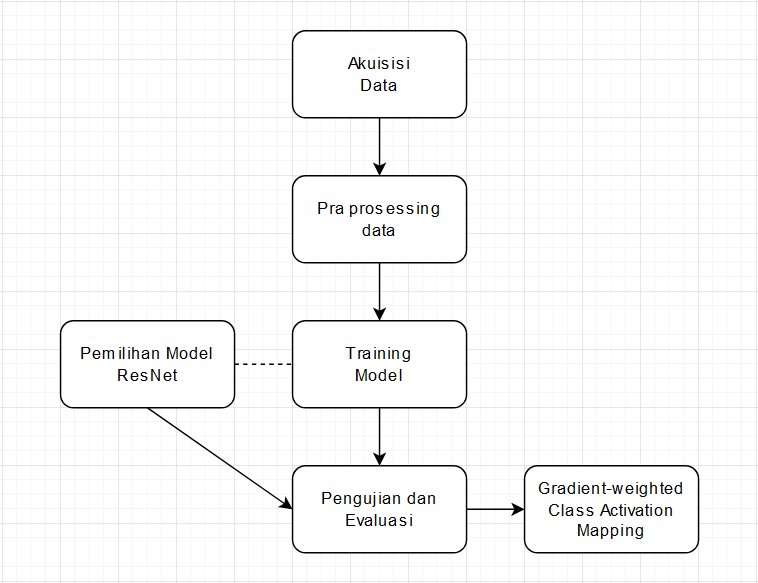
\includegraphics[scale=0.5]{gambar/diagramMethod.png}
	% Keterangan gambar yang diinputkan
	\caption{Diagram blok metodologi}
	% Label referensi dari gambar yang diinputkan
	\label{fig:diagramMethod}
\end{figure}

\subsection{Akuisisi Data}
\label{sec:321}
Data yang digunakan dalam penelitian ini adalah data yang diperoleh dari Diabetic Retinopathy Analisis Grand challenge \parencite{drac_challenge_2023_10280359}. Data yang digunakan adalah data citra retina yang sudah diberi label berupa tingkat keparahan penyakit retinopati diabetik yang sebelumnya sudah melalui proses image assesment sehingga sudah siap digunakan untuk training model. Dataset ini berisikan 611 citra OCT-A yang telah diberi label. Dataset ini juga berisikan 386 citra OCT-A yang tidak berlabel untuk dijadikan testing dataset.

\subsection{Pra-pemrosesan Data}
\label{sec:322}
Pra-pemrosesan data dilakukan untuk mempersiapkan data sebelum dilakukan proses pelatihan model. Pra-pemrosesan data yang dilakukan adalah konversi citra retina dari format .jpeg menjadi .png. Hal ini dilakukan karena format .png memiliki ukuran yang lebih kecil dibandingkan dengan format .jpeg. Selain itu, format .png juga tidak mengurangi kualitas citra retina. Pra-pemrosesan data juga dilakukan untuk membagi data menjadi data latih dan data uji. Data latih digunakan untuk melatih model sedangkan data uji digunakan untuk menguji model.

\subsection{Model ResNet}
\label{sec:323}
Model ResNet yang akan digunakan untuk dibandingkan dalam penelitian ini adalah model pre-trained resnet-18, resnet-34, resnet-50, resnet-101, dan resnet-152. Performa model-model tersebut akan dibandingkan dengan melihat nilai akurasi, \emph{loss}, dan \emph{val\_loss}.

\subsection{Pelatihan Model}
\label{sec:325}
Pelatihan model dilakukan dengan menggunakan metode \emph{transfer learning}. Metode \emph{transfer learning} dilakukan dengan menggunakan model ResNet yang sudah dipilih dan sudah dilatih dengan dataset ImageNet.
Arsitektur model yang digunakan sesuai pada penjelasan bagian \ref{sec:323} dengan menggunakan \emph{hyper-parameter} yang ada pada tabel \ref{tb:hyperParameterTraining}
\begin{table}[hbtp]
	\begin{center}
		\caption{Hyperparameter}
		\label{tb:hyperParameterTraining}
		\begin{tabular}{|
		>{\columncolor[HTML]{C0C0C0}}l |l|lll}
		\cline{1-2}
		Input shape                                         & 224,224,3      &  &  &  \\ \cline{1-2}
		Opimizer                                            & Adam           &  &  &  \\ \cline{1-2}
		Loss Function                                       & Cross Entropy  &  &  &  \\ \cline{1-2}
		Learning Rate                                       & 0.1            &  &  &  \\ \cline{1-2}
		Momentum                                            & 0.9            &  &  &  \\ \cline{1-2}
		\cellcolor[HTML]{C0C0C0}                            & Step size = 10 &  &  &  \\ \cline{2-2}
		\multirow{-2}{*}{\cellcolor[HTML]{C0C0C0}Scheduler} & Gamma = 0.1    &  &  &  \\ \cline{1-2}
		Epoch                                               & 100            &  &  &  \\ \cline{1-2}
		Batch size                                          & 32             &  &  &  \\ \cline{1-2}
		\end{tabular}
	\end{center}
\end{table}

\subsection{Pengujian dan Evaluasi}
\label{sec:326}
Pengujian dan evaluasi dilakukan dengan menggunakan data uji. Pengujian dan evaluasi dilakukan dengan melihat nilai akurasi, \emph{loss}, dan \emph{val\_loss}. Selain itu, pengujian dan evaluasi juga dilakukan dengan melihat \emph{confusion matrix} dari model yang sudah dilatih, untuk dilihat nilai presisi, recall, dan F1 pada setiap kelasnya, untuk melihat performa model dalam memprediksi tingkat keparahan penyakit retinopati diabetik.

\subsection{Gradient-weighted Class Activation Mapping}
\label{sec:327}
Grad-CAM digunakan untuk mengetahui faktor-faktor yang mempengaruhi model dalam memprediksi tingkat keparahan penyakit retinopati diabetik. Grad-CAM bekerja dengan menghitung gradien output model terhadap input, dan kemudian menggunakan gradien tersebut untuk memprediksi area input yang paling berkontribusi pada output model.